\documentclass{beamer}
\usepackage{amsmath, amssymb, amsbsy}
\usepackage{graphicx, subfigure}
%\usepackage[margin=1in,nohead]{geometry}
%\usepackage{siunitx}
%\usepackage{url}
%\usepackage{cite}

\usepackage{graphicx} % Allows including images
\usepackage{booktabs} % Allows the use of \toprule, \midrule and \bottomrule in tables

\setlength{\parindent}{0pt}
\setlength{\parskip}{12pt}

\newcommand{\uv}[1]{\ensuremath{{\hat{#1}}}} % for unit vector
\newcommand{\abs}[1]{\left| #1 \right|} % for absolute value
\newcommand{\avg}[1]{\left< #1 \right>} % for average
\let\underdot=\d % rename builtin command \d{} to \underdot{}
\renewcommand{\d}[2]{\frac{d #1}{d #2}} % for derivatives
\newcommand{\dd}[2]{\frac{d^2 #1}{d #2^2}} % for double derivatives
\newcommand{\pd}[2]{\frac{\partial #1}{\partial #2}} % for partial derivatives
\newcommand{\pdd}[2]{\frac{\partial^2 #1}{\partial #2^2}} % for double partial derivatives
\newcommand{\pdc}[3]{\left( \frac{\partial #1}{\partial #2}
\right)_{#3}} % for thermodynamic partial derivatives
\newcommand{\ket}[1]{\left| #1 \right>} % for Dirac bras
\newcommand{\bra}[1]{\left< #1 \right|} % for Dirac kets
\newcommand{\braket}[2]{\left< #1 \vphantom{#2} \right|\left. #2 \vphantom{#1} \right>} % for Dirac brackets
\newcommand{\matrixel}[3]{\left< #1 \vphantom{#2#3} \right|#2 \left| #3 \vphantom{#1#2} \right>} % for Dirac matrix elements
\newcommand{\grad}[1]{\gv{\nabla} #1} % for gradient
\let\divsymb=\div % rename builtin command \div to \divsymb
\renewcommand{\div}[1]{\gv{\nabla} \cdot #1} % for divergence
\newcommand{\curl}[1]{\gv{\nabla} \times #1} % for curl
\let\baraccent=\= % rename builtin command \= to \baraccent
\newcommand{\partder}[2]{\frac{\partial #1}{\partial #2}}
\newcommand{\material}[2]{\frac{D #1}{D #2}}
\newcommand{\tensor}[1]{\bar{#1}}
\newcommand{\tensplus}[3]{\tensor{#1}_{#2}^{#3}}

\mode<presentation> {

% The Beamer class comes with a number of default slide themes
% which change the colors and layouts of slides. Below this is a list
% of all the themes, uncomment each in turn to see what they look like.

%\usetheme{Berkeley}

\usetheme{Madrid}

}

%----------------------------------------------------------------------------------------
%	TITLE PAGE
%----------------------------------------------------------------------------------------

\title[]{Implementation of 1-D Vascular Model using Structured Tree Outflow Conditions} % The short title appears at the bottom of every slide, the full title is only on the title page

\author{Alex Baelde, Adam Updegrove, Debanjan Mukherjee} % Your name
%\institute[UCLA] % Your institution as it will appear on the bottom of every slide, may be shorthand to save space
%{
%University of California \\ % Your institution for the title page
%\medskip
%\textit{john@smith.com} % Your email address
%}
\date{\today} % Date, can be changed to a custom date

\begin{document}

\begin{frame}
\titlepage % Print the title page as the first slide
\end{frame}

\begin{frame}
\frametitle{Overview} % Table of contents slide, comment this block out to remove it
\tableofcontents % Throughout your presentation, if you choose to use \section{} and \subsection{} commands, these will automatically be printed on this slide as an overview of your presentation
\end{frame}

\section{Introduction}

\subsection{Project Goals}

%%%%%%%%%%%%%%%%%%%%%%%%%%%%%%%%%%%%%%%%%%%%%%%%%%%%%%%%%%%

\begin{frame}{Project Goals}

\begin{itemize}
	\item
	Use Olufsen's thesis to implement similar 1-D code in Matlab
	\item
	%These need to be filled in
	Investigate the effect of root impedance on blah
	\item
	%These need to be filled in
	Investigate blah on wave reflections
\end{itemize}


\end{frame}

%%%%%%%%%%%%%%%%%%%%%%%%%%%%%%%%%%%%%%%%%%%%%%%%%%%%%%%%%%

\begin{frame}{One-dimensional flow of blood - governing equations}
	\begin{block}{Continuity}
		\begin{equation}
			\label{continuity}
			\partder{A}{t} + \partder{q}{x} = 0
		\end{equation}
	\end{block}

	\begin{block}{Conservation of X Momentum}
		\begin{equation}
			\label{consxmomentum}
			\partder{q}{t} + \partder{}{x}\Bigg(\frac{q^2}{A}\Bigg) + \frac{A}{p}\partder{p}{x} = -\frac{2R\pi \nu q}{\delta A}
		\end{equation}
	\end{block}
	
\end{frame}


%%%%%%%%%%%%%%%%%%%%%%%%%%%%%%%%%%%%%%%%%%%%%%%%%%%%%%%%%%%
\section{Implementation}
\subsection{Discretization}

\begin{frame}{Numerical Solution $\&$ Development of a Code}
\footnotesize
		\begin{block}{}
		A Two-Step Lax-Wendroff (Richtmyer) scheme is used. Equations~\ref{continuity} and \ref{consxmomentum} can be written in the following form:

		\begin{equation} 
			\label{discrete1}
			\partder{}{t} \tensor{U} + \partder{}{x} \tensor{R}(\tensor{U}) = \tensor{S}
		\end{equation}
		\end{block}
		
			\begin{equation*}
		\label{bigu1}
		\tensplus{U}{j}{T+1} = \tensplus{U}{j}{T} - \frac{k}{h} \Bigg(\tensplus{R}{j+1/2}{T+1/2} - \tensplus{R}{j-1/2}{T+1/2} \Bigg) + \frac{k}{2} \Bigg(\tensplus{S}{j		+1/2}{T+1/2} + \tensplus{S}{j-1/2}{T+1/2} \Bigg)
	\end{equation*}
	
		\begin{align*}
		\tensplus{U}{j}{T+1/2} &= \frac{\tensplus{U}{j+1/2}{T} + \tensplus{U}{j-1/2}{T}}{2} + \frac{k}{2h} \Bigg(-\tensplus{R}{j+1/2}{T} - \tensplus{R}{j-1/2}{T} \Bigg)\\ 		&+ \frac{k}{4} \Bigg(\tensplus{S}{j+1/2}{T} + \tensplus{S}{j-1/2}{T} \Bigg)
		\end{align*}
\end{frame}

%%%%%%%%%%%%%%%%%%%%%%%%%%%%%%%%%%%%%%%%%%%%%%%%%%%%%%%%%%%

\begin{frame}{Hyperbolic system and finite difference discretization}
\footnotesize

	\begin{equation*}
		\label{bigu1}
		\tensplus{U}{j}{T+1} = \tensplus{U}{j}{T} - \frac{k}{h} \Bigg(\tensplus{R}{j+1/2}{T+1/2} - \tensplus{R}{j-1/2}{T+1/2} \Bigg) + \frac{k}{2} \Bigg(\tensplus{S}{j		+1/2}{T+1/2} + \tensplus{S}{j-1/2}{T+1/2} \Bigg)
	\end{equation*}
	
		\begin{align*}
		\tensplus{U}{j}{T+1/2} &= \frac{\tensplus{U}{j+1/2}{T} + \tensplus{U}{j-1/2}{T}}{2} + \frac{k}{2h} \Bigg(-\tensplus{R}{j+1/2}{T} - \tensplus{R}{j-1/2}{T} \Bigg)\\ 		&+ \frac{k}{4} \Bigg(\tensplus{S}{j+1/2}{T} + \tensplus{S}{j-1/2}{T} \Bigg)
		\end{align*}

\end{frame}

%%%%%%%%%%%%%%%%%%%%%%%%%%%%%%%%%%%%%%%%%%%%%%%%%%%%%%%%%%%

\subsection{Inflow}
\begin{frame}{Inflow profile and inlet boundary condition}

\begin{figure}[ht]
	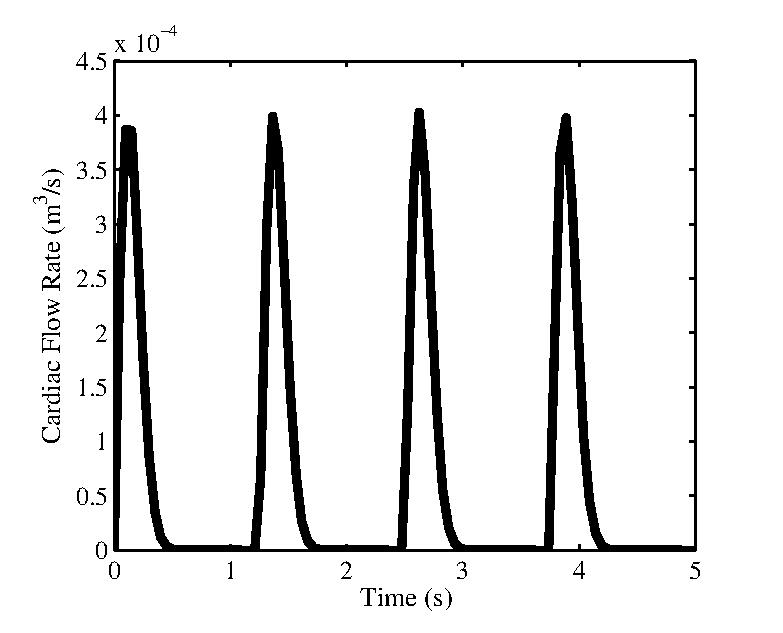
\includegraphics[width=3.75in]{inflow}
	\label{inflower}
	\caption{The inflow profile from measured data in $m^3/s$. The curve is measured at the upper ascending aorta using magnetic resonance.}
\end{figure}

\end{frame}

%%%%%%%%%%%%%%%%%%%%%%%%%%%%%%%%%%%%%%%%%%%%%%%%%%%%%%%%%%%
\subsection{Outflow}
\begin{frame}{The structured tree}
	\begin{block}{Olufsen's}
		She retains no structure of the vessels within the tree and recalculates all this information for each structured tree.	
		\begin{equation}
			\label{radius}
			(r_0)_(n,k) = R_{root} \alpha^k\beta^{n-k}
		\end{equation}
	\end{block}
	
	\begin{block}{Our's}
		We retain a structure of the tree by a vector of nodes containing certain information about the tree. 
		\begin{equation}
			\begin{bmatrix}
			Daughter \: 1 \; & Daughter \: 2 \; & Parent \; & Radius 
			\end{bmatrix}
		\end{equation}
	\end{block}
		
\end{frame}

%%%%%%%%%%%%%%%%%%%%%%%%%%%%%%%%%%%%%%%%%%%%%%%%%%%%%%%%%%%

\begin{frame}{Outflow boundary condition using structured tree}
\begin{block}{Method of Characteristics}
	 \begin{equation}
 		\label{characteristics}
 		\Gamma_{+/-}\; : A_Q - A_{R/S} + \frac{Q_Q - Q_{R/S}}{-(Q_{R/S}/A_{R/S}) + C_R} = H_{R/S}^{+/-} \Delta t
	\end{equation}
\end{block}

\begin{figure}[ht]
	\centering
	\label{characteristicplot}
	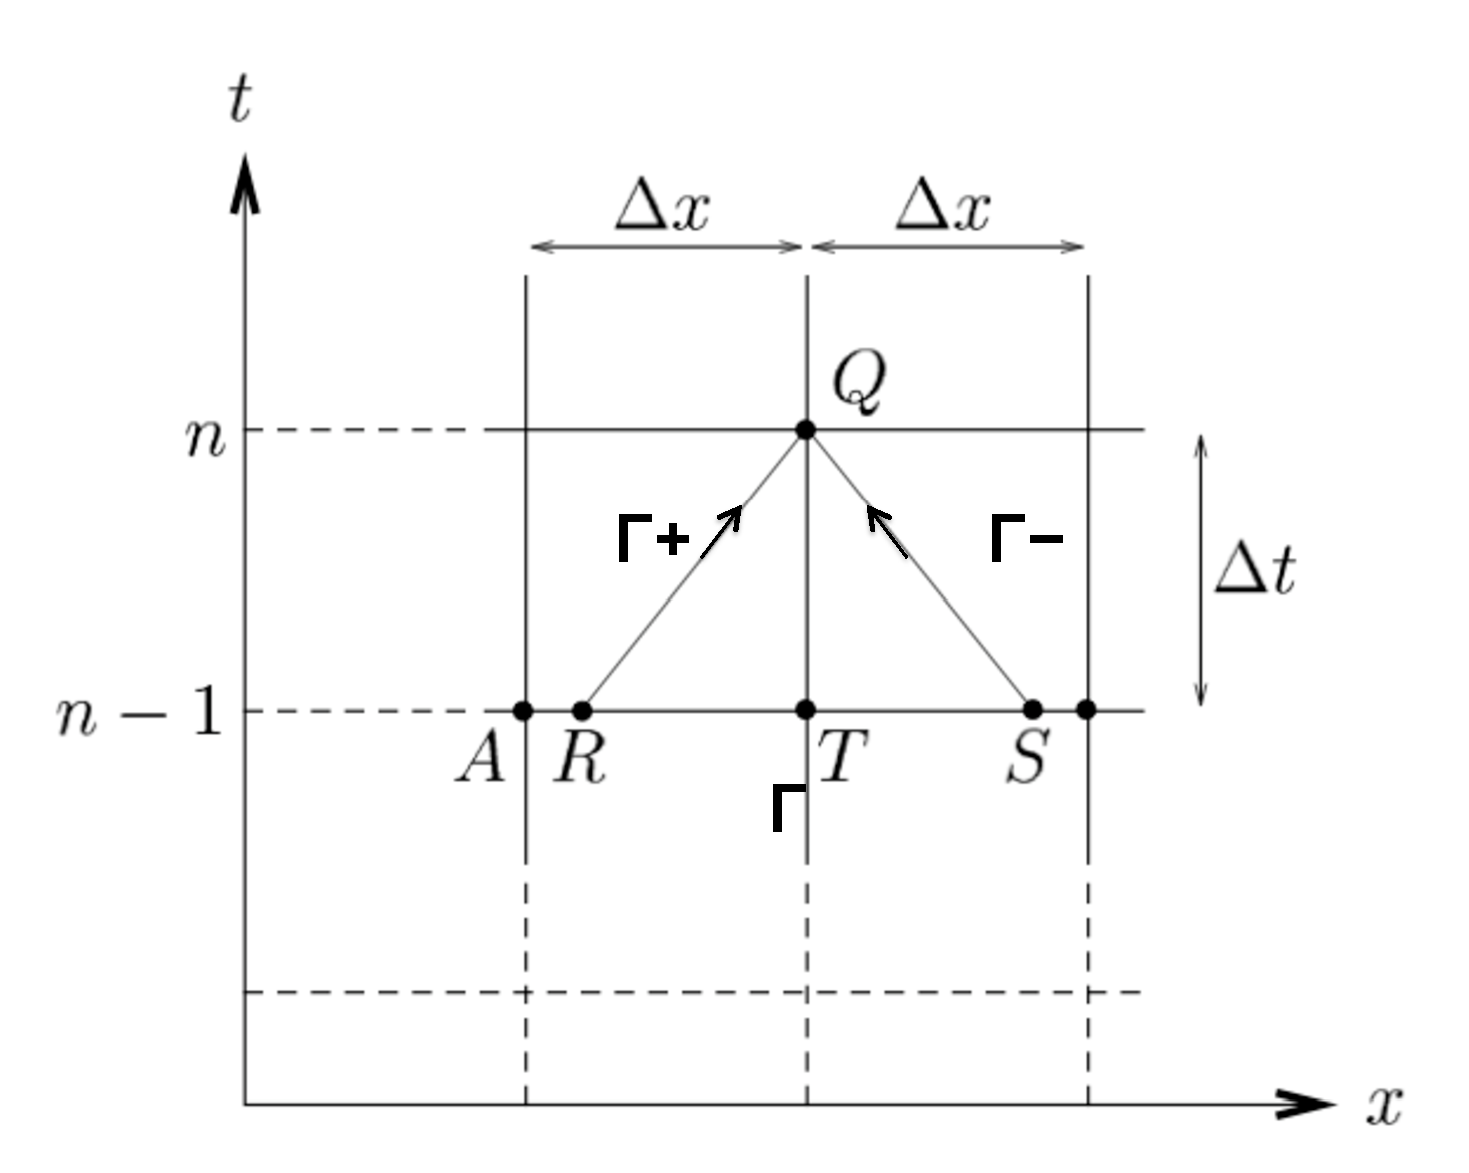
\includegraphics[width=2in]{characterplot}
\end{figure}

\end{frame}

%%%%%%%%%%%%%%%%%%%%%%%%%%%%%%%%%%%%%%%%%%%%%%%%%%%%%%%%%%%
\section{Results}

\subsection{Our Implementation}
\begin{frame}{Toy problem for comparison}

\begin{block}{Single Tube with Resistance Boundary Condition}
	The pressure profile follows the same curve. The dicrotic notch is less visible in our implementation, and the magnitude is slightly higher. 
\end{block}

\begin{figure}[ht]
	\centering
	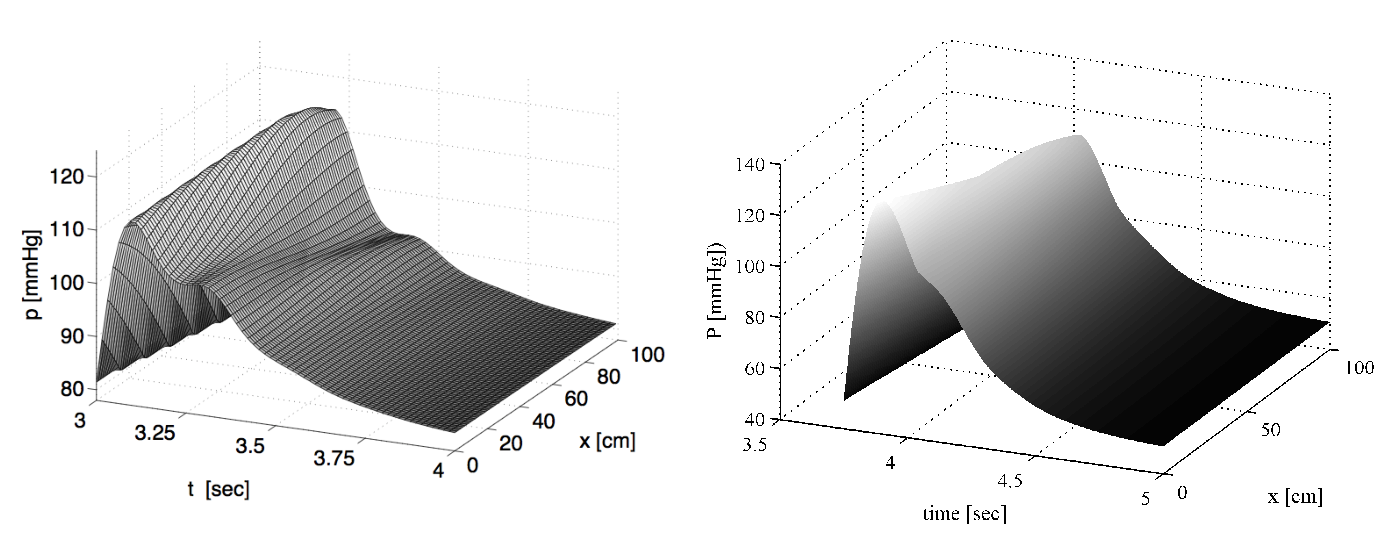
\includegraphics[width=4.5in]{pplot}
	\label{ours}
\end{figure}

\end{frame}

\begin{frame}{Toy problem for comparison}
\begin{block}{Single Tube with Structured Tree Boundary Condition}
	The pressure profile follows the same curve. The dicrotic notch is less visible in our implementation, and the magnitude is slightly higher. 
\end{block}
\vspace{-1.0cm}
\begin{figure}[ht]
	\centering
	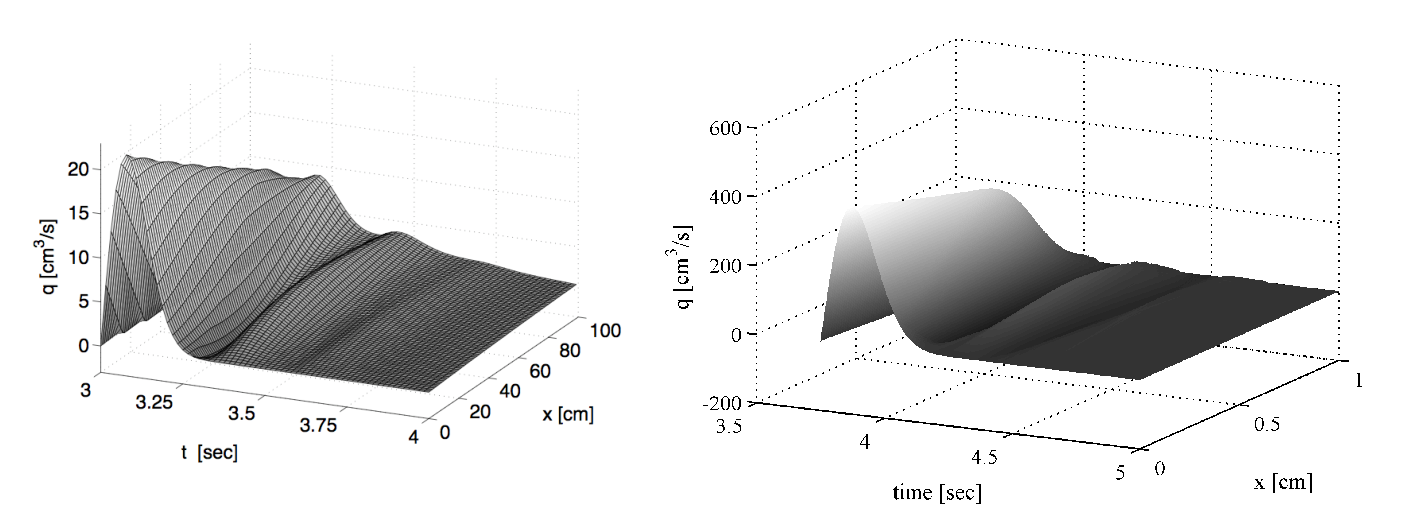
\includegraphics[width=5.0in]{qplot-crop.pdf}
	\label{ours}
\end{figure}

\end{frame}

%%%%%%%%%%%%%%%%%%%%%%%%%%%%%%%%%%%%%%%%%%%%%%%%%%%%%%%%%%%

\begin{frame}
	\begin{center}
		\Large{\textbf{Flow analysis: What information can we get from such 1-dimensional, reduced order models ?}}
	\end{center}
\end{frame}

%%%%%%%%%%%%%%%%%%%%%%%%%%%%%%%%%%%%%%%%%%%%%%%%%%%%%%%%%%%
\subsection{Olufsen Implementation}

\begin{frame}{Wave reflection phenomena - comparison with Windkessel models}

\begin{center}
\textbf{This was discussed in detail during the Journal Club review of the paper}
\end{center}

\end{frame}

%%%%%%%%%%%%%%%%%%%%%%%%%%%%%%%%%%%%%%%%%%%%%%%%%%%%%%%%%%%

\begin{frame}{Varying terminal resistance of tree for flow regulation}

	\begin{columns}
		\begin{column}[r]{5.5cm}
			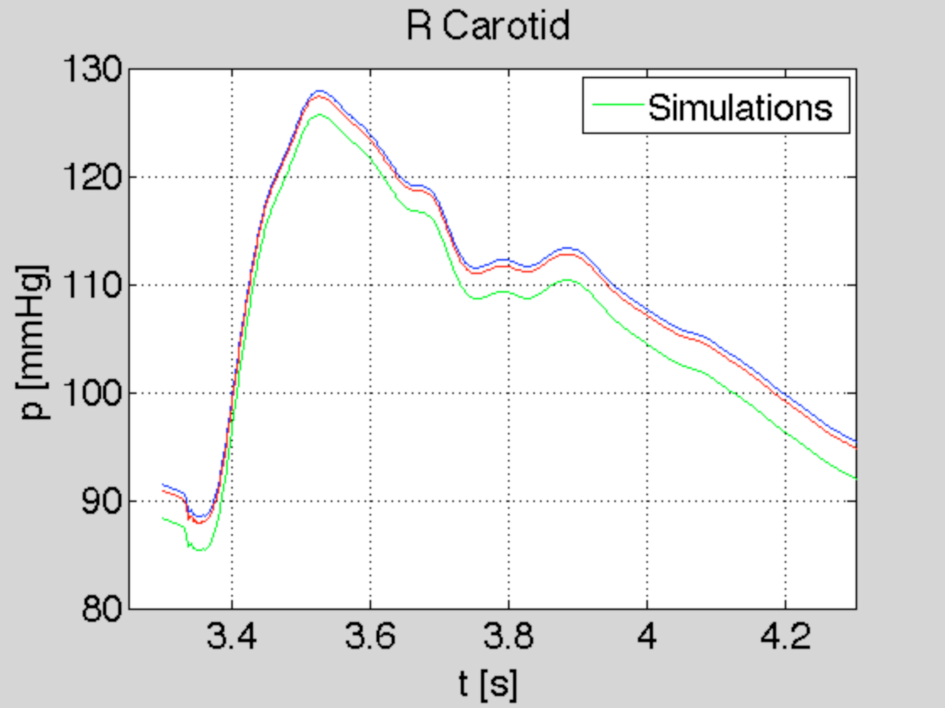
\includegraphics[width=5.5cm]{pcarotid.pdf}
		\end{column}
		\begin{column}[l]{5.5cm}
			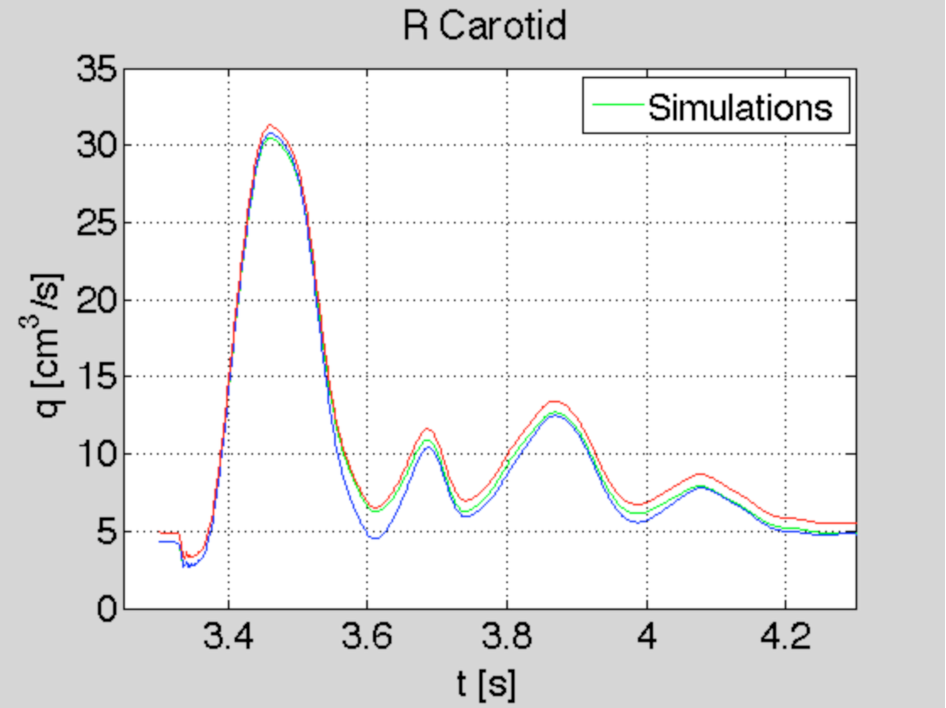
\includegraphics[width=5.5cm]{qcarotid.pdf}
		\end{column}
	\end{columns}
	
	\begin{center}
		\footnotesize
		\textbf{increased terminal resistance from 0 (in green) to $\mathbf{230000\,\,dynes-s/cm^5}$ (in blue) in all vascular beds, and then reduced terminal resistance to 0 in R. Carotid to regulate flow (in red).}
	\end{center}

\end{frame}

%%%%%%%%%%%%%%%%%%%%%%%%%%%%%%%%%%%%%%%%%%%%%%%%%%%%%%%%%%%

\begin{frame}{Radius of large vessels - insights on stenosis/aneurysms ?}

	\begin{columns}
		\begin{column}[r]{5.5cm}
			\centering
			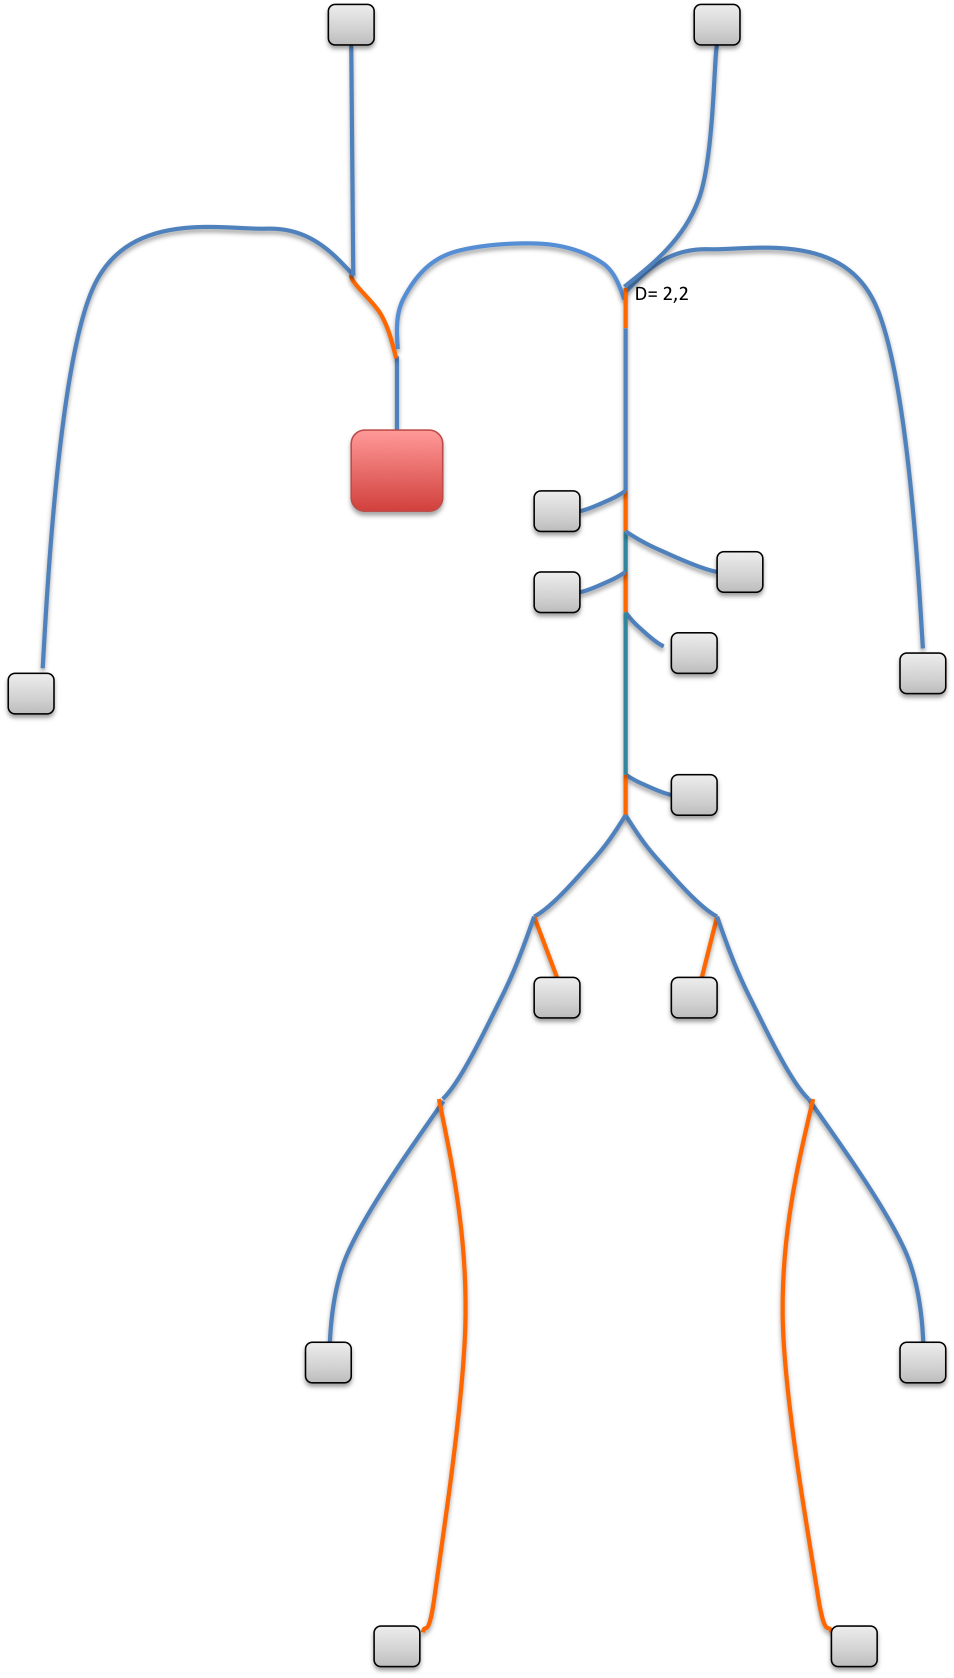
\includegraphics[width=3.75cm]{fulltree.png}\\
			\textbf{\footnotesize{A modified version of the vascular tree for studying vessel radius effects}}
		\end{column}
		\begin{column}[l]{5.5cm}
			\begin{block}{\footnotesize{Modifications to the vessel radii}}
		
			\end{block}
		\end{column}
	\end{columns}

\end{frame}

\begin{frame}{Radius of large vessels - insights on stenosis/aneurysms}

	\begin{center}
	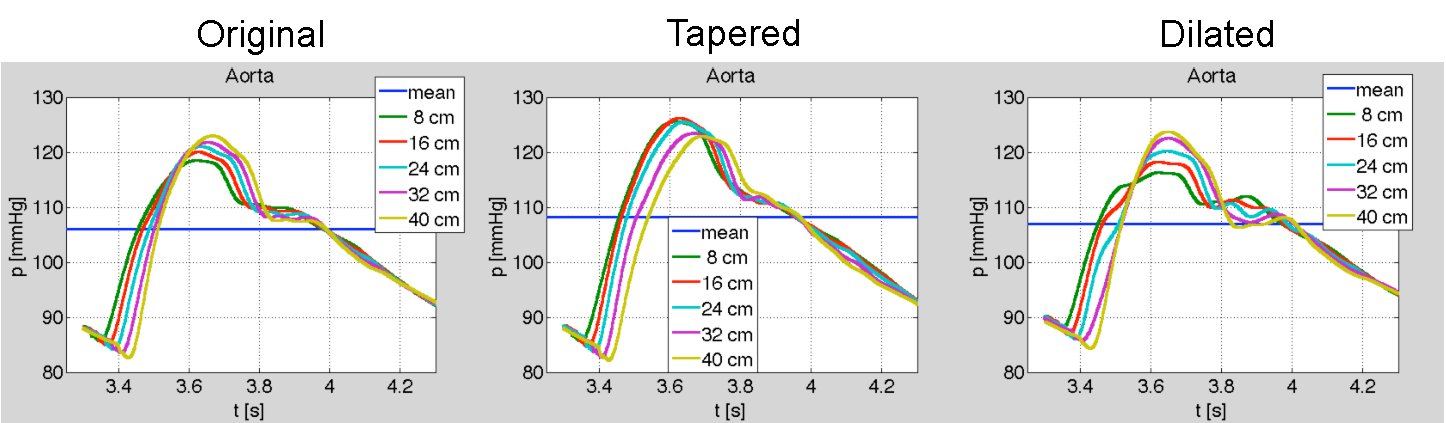
\includegraphics[width=11.0cm]{aortawavereflections.pdf}
	\end{center}

\end{frame}

%%%%%%%%%%%%%%%%%%%%%%%%%%%%%%%%%%%%%%%%%%%%%%%%%%%%%%%%%%%
\section{Discussion and Conclusion}

\begin{frame}{Concluding remarks}
\begin{itemize}
	\item
	Currently implemented way is not always the best way.
	\item
	%Fill in here!
	Something else
\end{itemize}
\end{frame}

\end{document}
